\chapter{Testautomatisierung}
\label{sec:testautomatisierung}
In Kapitel \ref{sec:testautoGrundlagen} wurde der Begriff Testautomatisierung bereits eingeführt. Die darin gewählte Definition hat gezeigt, dass man unter Testautomatisierung weit mehr versteht, als das automatisierte ausführen von Testfällen auch wenn das der wohl am weitesten verbreiteten Bereich der Automatisierung ist.
Testautomatisierung ist in allen Bereichen des Entwicklungs- bzw. Testprozesses möglich.
\glqq Das Spektrum umfasst alle Tätigkeiten zur Überprüfung der Softwarequalität im Entwicklungsprozess, in den unterschiedlichen Entwicklungsphasen und Teststufen so wie die entsprechenden Aktivitäten von Entwicklern, Testern, Analytikern oder auch der in die Entwicklung eingebundenen Anwender. Die Grenzen der Automatisierung liegen darin, dass diese nur die manuellen Tätigkeiten eines Testers übernehmen kann, nicht aber die intellektuelle, krative und intuitive Dimension dieser Rolle.\grqq\ \cite[S. 7]{seidl_basiswissen_2012}
Die intellektuelle Dimension ist vor allem in den frühen Phasen des Testprozesses gefordert. Diese Phasen sind maßgeblich für die Spätere Qualität der einzelnen Testfälle. Testautomatisierung wird daher nie die arbeiten eines guten Testanalysten voll ersetzen können. Um so weiter der Testprozess voranschreitet, um so praktischer werden auch die zu erledigenden Aufgaben. Das Potential für eine Automatisierung steigt also im laufe des Testprozesses.
Fewster und Graham stellen diesen Zusammenhang in einer Grafik bildlich dar. \cite[vgl. S.18]{fewster_software_1999} Abbildung \ref{fig:intellektuellVsPraktisch} greift diese Darstellung auf und passt sie auf den in Kapitel \ref{sec:testprozess} vorgestellten Testprozess an. Die verschiedenen Möglichkeiten der Testautomatisierung werden in Kapitel \ref{sec:bereiche_der_estautomatisierung} geklärt. Zunächst soll jedoch die Frage beantwortet werden warum eine Automatisierung von Testfällen überhaupt Sinn macht.

\begin{figure}[htb]
  \centering  
  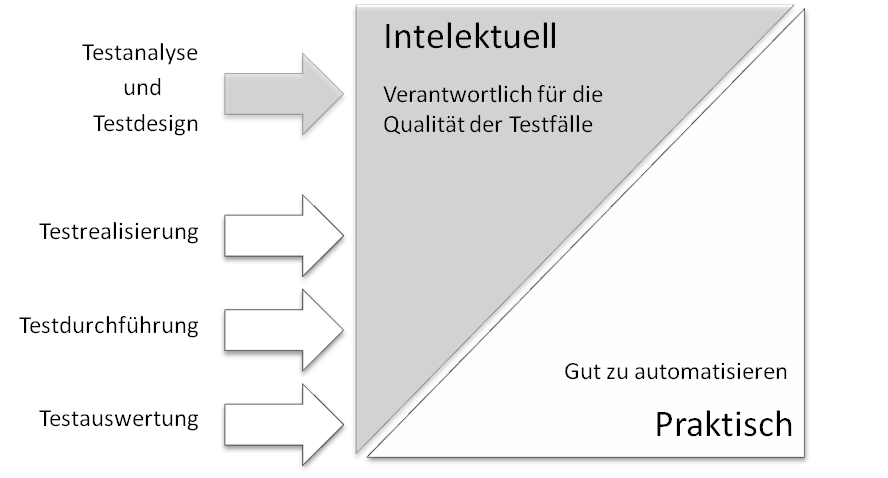
\includegraphics[scale=1]{img/intelektuellVsPraktisch.png}\\
  \footnotesize\sffamily\textbf{Quelle:} \cite[vgl. S.18]{fewster_software_1999}
  \caption{Grenzen und Möglichkeiten der Testautomatisierung}
  \label{fig:intellektuellVsPraktisch}
\end{figure}

\section{Warum Testautomatisierung}
\label{sec:warum_testautomatisierung}

Richtig durchgeführt kann Testautomatisierung eine Reihe von Vorteilen bringen. Dustin et al. stellen drei bedeutende Vorteile der Testautomatisierung fest. \cite[S.44 ff.]{dustin_software_2001}
\begin{itemize}
\item[1.] Erstellung eines zuverlässigen Systems
\item[2.] Verbesserung der Testqualität und Testtiefe
\item[3.] Verringerung des Testaufwands und Reduzierung des Zeitplans
\end{itemize}


In der Literatur gibt es zahlreiche Listen von Vorteilen der Testautomatisierung die sehr viel feiner gegliedert sind als die von Dustin et al. gewählten Oberpunkte. \cite{fewster_software_1999} \cite{thaller_software-test_2002}
Gleicht man diese Vorteile mit den von Dustin et al. gewählten Oberpunkten ab zeigt sich, dass vor allem die Punkte 2 und 3 gut durch diese repräsentiert werden. Sie lassen sich leicht mit den feiner ausformulierten Vorteilen unterfüttern. Die Erstellung eines zuverlässigen Systems ist hingegen nur schwer direkt zu beeinflussen. In der Regel wird dieser Punkt indirekt durch eine Verbesserung in in den Punkten 2 und 3 beeinflusst.
Eine Verringerung des Testaufwands für einzelne Tests schafft mehr Zeit die in bessere und breiter angelegte Tests investiert werden kann. Neben der direkten Beeinflussung führt Testautomatisierung also zusätzlich auch indirekt zu einer höhere Testqualität und Testtiefe. Diese bedingt dann wiederum dass mehr Fehler im System aufgedeckt werde können. So kann eine höhere Qualität des Endproduktes erreicht werden die sich in einem zuverlässigeren System zeigt.
Auf Grund seiner passiven Natur wird Punkt 1 daher im weiteren nicht näher betrachtet.
Fewster und Graham fassen die Vorteile der Testautomatisierung noch weiter zusammen und reduzieren sich in ihrer Fazit auf die Worte Qualitäts- und Effizienzsteigerung.
Diese Begriffe entsprechen weitestgehend den von Dustin et al. gewählten Oberpunkten. Qualitätssteigerung fasst dabei die Verbesserung der Testqualität und Testtiefe zusammen, die Verringerung des Testaufwands und Reduzierung des Zeitplans entspricht der Effizienzsteigerung. 
Um die Vorteile der Testautomatisierung auf eine Feinere und damit greifbarer Ebene zu bewegen werden im Folgenden die Vorteile wie sie 
Fewster und Graham beschreiben verwendet und den von Dustin et al. gewählten Kategorien zugeordnet.

\subsection{Verringerung des Testaufwands und Reduzierung des Zeitplans}
\label{sec:verringerung_des_testaufwands_und_reduzierung_des_zeitplans}
Die Vorteile in Tabelle \ref{tbl:effizienz_testautomatisierung} beschreiben, dass der Aufwand der für das Testen einer Software betrieben werden muss mit Hilfe von Automatisierung reduziert werden kann.
Reduzierter Aufwand in den Tests so wie eine schnellere und wiederholbare Abarbeitung der Testfälle führen dann meist dazu, dass der gesamte Zeitplan des Projekts positiv beeinflusst wird. Sein volles Potential entfaltet Automatisierung immer dann, wenn Testfälle wiederholt ausgeführt werden. Regressionstests, die vor jedem neuen Releaszyklus einer Software ausgeführt werden sind daher beispielsweise prädestiniert dazu automatisiert zu werden. Tester können so von sich wiederholenden Testaufgaben entlastet werden. Der Testaufwand wird reduziert und die Tester sind frei für andere Aufgaben was wiederum das Projekt beschleunigt.

\begin{table}
\begin{tabular}{p{0.4\textwidth}|p{0.6\textwidth}}
Ausführen existierender Regressionstests für eine neue Version der Software
& Der Aufwand um Regressionstests manuell durchzuführen kann schnell sehr groß werden. Sind Testfälle automatisiert ist es möglich sie bei Änderungen am System mit wenig aufwand erneut durchzuführen. \\
\hline 
Besserer Einsatz von Resourcen
& Durch Automatisierung lässt es sich vermeiden Tester mit generischen Aufgaben zu binden wie beispielsweise das immer gleiche Tippen von Testeingaben.
Die so freien gewordenen Resourcen können für andere Aufgaben verwendet werden.
Der Zeitplan des Projektes kann so verkürzt werden. \\ 
\hline 
Wiederverwendbarkeit von Testfällen & 
Neue Projekte können von den Ergebnissen der Testautomatisierung aus vorangegangenen Projekten profitieren. Auch innerhalb eines Projektes können Teile von Automatisierten Testfällen oft wiederverwendet werden.
Das Reduziert den Zeitplan des Projekts. \\ 
\hline 
Frühere Markteinführung. & Richtig eingesetzt beschleunigt Testautomatisierung den gesamten Testprozess. Das verkürzt letztendlich auch die Zeit bis zur Markteinführung der Software. \\ 


\end{tabular} 
\caption{Verringerung des Testaufwands und Reduzierung des Zeitplans nach Fewster und Graham \cite[vgl. S. 9 ff.]{fewster_software_1999}}
\label{tbl:effizienz_testautomatisierung}
\end{table}

\subsection{Verbesserung der Testqualität und Testtiefe}
\label{sec:verbesserung_der_testqualität_und_testtiefe}
Die in Tabelle \ref{tbl:qualitaet_testautomatisierung} beschriebenen Vorteile zeigen, dass sich mit Hilfe der Testautomatisierungen Verbesserungen im Bereich der Testqualität und Testtiefe erreichen lassen. Eine bessere Testqualität wird meist dadurch erzielt, dass die Testfälle in ihrer Gesamtheit ein höheres Potential erreichen Fehler aufzudecken. Eine hohe Testtiefe und eine möglichst breite Testabdeckung bedingen daher eine allgemein höhere Qualität der Tests. Aber auch die Qualität einzelner Testfälle kann mittels Testautomatisierung direkt verbessert werden. Vor allem eine bessere Wiederverwendbarkeit und Wiederholbarkeit sind hier der ausschlaggebende Faktor.

\begin{table}
\begin{tabular}{p{0.4\textwidth}|p{0.6\textwidth}}
\\
\hline 
Mehr Testfälle öfter ausführen
& Aus Zeitmangel müssen sich Tester oft auf einen geringeren Testumfang zurückziehen also eigentlich gewünscht ist. Vor allem bei sehr generischen Testfällen, die sich vielleicht nur in verschiedenen Maskeneingabe unterscheiden ist es mithilfe von Testautomatisierung möglich in weniger Zeit ein vielfaches an Testfällen durchzuführen.
Eine tiefere Testabdeckung ist die Folge. Da solche Testfälle in der Regel auf einem generischen Basistestfall beruhen ist es hier besonders einfach möglich eine durchgehend hohe Testqualität zu gewährleisten. \\ 
\hline 
Testfälle durchführen die ohne Automatisierung schwer bis unmöglich wären & 
Einen Lasttest für mit z.B. mehr als 200 Benutzern manuell durchzuführen erweist sich als nahezu unmöglich. Die eingaben von 200 Benutzern lassen sich mit Hilfe von automatisierten Lasttests jedoch gut simulieren. Über Testfälle die ohne Automatisierung gar nicht möglich wären, lässt sich die Testbreite erhöhen. Die Qualität der Tests steigt durch das erhöhte Potential Fehler zu entdecken. \\ 
\hline 
Konsistenz und Wiederholbarkeit von Testfällen & Testfälle die automatisch durchgeführt werden, werden immer auf die selbe weise durchgeführt. Eine derartige Konsistenz in den Testfällen ist auf Manuellem Wege kaum zu erreichen. Fehlerhaft in der Testfalldurchführung können so vermieden werden. Die Qualität der Testfälle steigt. \\ 
\hline 
Erhöhtes Vertrauen in die Testfälle und Software & Das Wissen, dass eine vielzahl an Testfällen erfolgreich vor jedem Release durchgeführt wurde, erhöht das vertrauen von Entwickler und Kunden, dass unerwartete Überraschungen ausbleiben.
Werden Testfälle regelmäßig ausgeführt, erhöht das zusätzlich das vertrauen, dass diese Testfälle stabil sind und keine Falschmeldungen liefern. \\ 


\end{tabular} 
\caption{Verbesserung der Testqualität und Testtiefe nach Fewster und Graham \cite[vgl. S. 9 ff.]{fewster_software_1999}}
\label{tbl:qualitaet_testautomatisierung}
\end{table}

\subsection{Kosten also Bewertungsgrundlage für die Testautomatisierung}
\label{sec:kosten_der_testautomatisierung}
Die unter Kapitel \ref{sec:verbesserung_der_testqualität_und_testtiefe} und Kapitel \ref{sec:verringerung_des_testaufwands_und_reduzierung_des_zeitplans} aufgezeigten Vorteile eignen sich gut um sich in einer Diskussion über das testen positiv über eine Automatisierung zu äußern. Die genannten Argumente haben allerdings das große Problem, dass sie sich meist nur schwer messen und mit genauen Zahlen belegen lassen.
Um das zu erreichen muss man sich auf die kleinste gemeinsame Größe zurückziehen auf die all die genannten Vorteile hinarbeiten: Eine Reduzierung der Kosten beim Testen.
Sowohl eine Verbesserung der Testqualität und Testtiefe als auch eine Verringerung des Testaufwands und Reduzierung des Zeitplans verfolgen in letzter Instanz immer das Ziel Kosten einzusparen. Sei es direkt durch z.B. eine verkürzte Projektlaufzeit als auch indirekt durch geringere Folgekosten in der Wartung bedingt durch eine höhere Testqualität.
Letzteres ist wiederum schwer mit einer genauen Zahl zu beziffern. Ist ein Projekt erst einmal abgeschlossen lässt sich nicht mehr einfach ermitteln wie hoch die Differenz und der Schweregrad der gefundenen Fehler beim automatisierten im Gegensatz zum manuellen Testen wäre.
Um den Nutzen von Testautomatisierung daher für ein Projekt nachvollziehbar zu begründen bieten die direkten Kosten die durch das erstellen und ausführen der Testfälle entstehen den besten Angriffspunkt. \cite{ramler_economic_2006}
Ramler und Wolfmaier \cite{ramler_economic_2006} zitieren eine Fallstudie von Linz und Daigl \cite{dustin_automated_1999} die eine Unterteilung der Kosten in Zwei Komponenten vornimmt.
\begin{itemize}
    \item[] \(V:=\text{Ausgaben für testspezifikation und implementierung}\)
    \item[] \(D:=\text{Ausgaben für eine einzelnen Testlauf}\)
\end{itemize}

Mit Hilfe dieser beiden Variablen können die Kosten (\(A_a\)) für einen einzelnen automatisierte Testfall wie folgt angegeben werden:
\begin{equation}
A_a:=V_a+n*D_a
\end{equation}
\(V_a\) Symbolisiert die Kosten die für die Spezifikation und Implementierung des automatisierten Testfalls anfallen. \(D_a\) die Kosten die für das einmalige Ausführen des Testfalles entstehen und \(n\) für die Anzahl der durchgeführten Testläufe.
Um zu bestimmen wie sich das Manuelle und Automatisiertes Testen zueinander verhalten, kann analog die selbe Gleichung für das manuelle Testen aufgestellt werden.
\begin{equation}
A_m:=V_m+n*D_m
\end{equation}

Mit Hilfe dieser beiden Gleichungen lässt sich zeigen, dass sich ab einer gewissen Anzahl an Testläufen die Automatisierung gegenüber der manuellen Ausführung aus Sicht der Kosten lohnt.
Es wird dabei davon ausgegangen, dass die initiale Investition \(V_a\) für die Automatisierung höher ist als die initiale Investition für das Manuelle Testen \(V_m\).
Die Kosten des Testfalls steigen mit jeder Testausführung \(n\) für die Automatisierung jedoch langsamer an. Beide Funktionen schneiden sich daher in einem break-even Punkt ab dem die Automatisierung die günstigere Alternative darstellt.
Abbildung \ref{fig:breakEven} veranschaulicht diesen Zusammenhang noch einmal grafisch.

\begin{figure}[htb]
  \centering  
  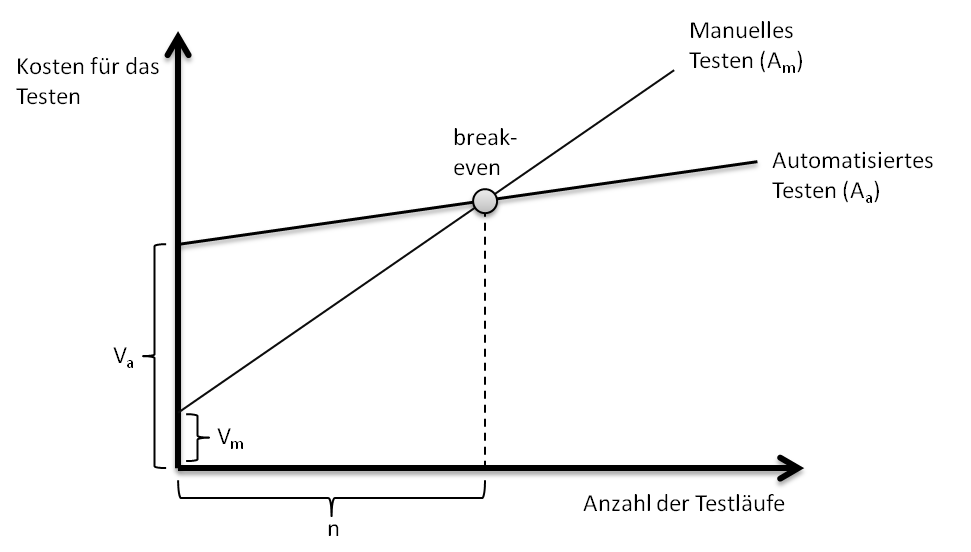
\includegraphics[scale=0.8]{img/breakeven.png}\\
  \footnotesize\sffamily\textbf{Quelle:} \cite{ramler_economic_2006}
  \caption{Break-even Punkt für Testautomatisierung}
  \label{fig:breakEven}
\end{figure}

Zusammenfassend lässt sich also feststellen, dass vor allem wiederholt ausgeführte Testtätigkeiten hohes Einsparungspotential bei einer Testautomatisierung bieten.


\subsection{Probleme der Testautomatisierung}
\label{sec:probleme_der_testautomatisierung}
Ramler und Wolfmaier \cite{ramler_economic_2006} zitieren ein erreichen des break-even Punkt wie er in Kapitel \ref{sec:kosten_der_testautomatisierung} beschrieben ist nach einer Ausführung von 2-20 Testläufen. Diese große Spanne macht noch einmal deutlich, wie wichtig es ist in der Testplanung und Steuerung genau abzuwägen ob und wo eine Automatisierung sinnvoll einzusetzen ist. Eine Automatisierung kann oft auch unwirtschaftlich sein, vor allem immer dann, wenn Tests nur ein einziges mal ausgeführt werden. Implementierungs- und Wartungsaufwand von automatisierten Testfällen sind meist sehr viel höher als die von Manuellen Testfällen. Dieser Mehraufwand muss in irgend einer weise gerechtfertigt sein. Oftmals wird dieser Punkt vernachlässigt und die Testautomatisierung als Heilmittel für schlecht laufende Prozesse und zu hohe Kosten gesehen. Dabei ist genau das Gegenteil der Fall. Es ist sinnvoller zunächst die Qualität der Tests und des eigenen Testprozesses zu optimieren bevor eine Automatisierung eingeführt wird. 
Eine weiterer Schwachpunkt der Automatisierung ist nach Fewster und Graham \cite[vgl. S. 22 ff.]{fewster_software_1999}, dass die Automatisierung von Software-Tests zwar einen deutlichen Mehraufwand bedeuten jedoch die Anzahl der gefundenen Fehler nur gering erhöht wird.
Bevor Testfälle automatisiert werden, müssen sie in der Regel zuvor einmal manuell durchgeführt werden um sicher zu stellen, dass der angedachte Test auch sinnvoll und realisierbar ist. Meist werden Fehler bereits bei dieser manuellen Aufgabe festgestellt. Wird der Testfall dann automatisiert, deckt er weit weniger wahrscheinlich einen Fehler auf als bei seiner ersten, manuellen Ausführung. Darüber hinaus können automatisierte Testfälle Fehler nur über die Akzeptanzkriterien aufdecken die ihnen explizit hinterlegt wurden. Oft reichen die hinterlegten Kriterien aber nicht aus um alle Fehlerquellen abzudecken. Das kann dazu führen, dass Testfälle als positiv gekennzeichnet werden obwohl sie in Wirklichkeit fehlerhaft waren. Bei manuellen Tests fallen vergessene Akzeptanzkriterien eher auf bzw. werden durch den Tester instinktiv hinzu gedacht. Die Anzahl der fälschlicherweise positiv gewerteten Testfälle sinkt. Eine weitere positiven Aspekt den ein manueller Tester mit sich bringt ist eine höhere Stabilität in den Testfällen. Ein Tester kann sich auf kleinere Änderungen in der zu testenden Software leicht einstellen. Er kann selbst entscheiden ob eine Abweichung vom Testfall als Fehler zu werten oder zu vernachlässigen ist. Automatisierte Testfälle bieten diesen Luxus nicht. Sie verfolgen einen festen Ablaufplan und können nur schwer mit Veränderungen in der zu testenden Software umgehen. Das macht sie im Vergleich zu manuellen Tests instabil und erfordert einen erhöhten Wartungsaufwand. In manchen Fällen kann diese Abhängigkeit zwischen Software und automatisiertem Test sogar so weit führen, dass sie die Entwicklung der Software behindern. Beispielsweise dann, wenn eine Änderung in der Software so große Auswirkungen auf die automatisierten Testfälle hätte, dass es aus wirtschaftlicher Sicht nicht mehr sinnvoll ist sie durchzuführen. Die Kosten für die Anpassungen an den Tests wären dann so hoch, dass sie den Nutzen, welchen die Änderung an der Software bringt nicht mehr aufwiegen kann. \cite[vgl. S. 22 ff.]{fewster_software_1999}
Analog zu den in Tabelle \ref{tbl:effizienz_testautomatisierung} und \ref{tbl:qualitaet_testautomatisierung} genannten Vorteilen haben Fewster und Graham \cite[vgl. S. 10 ff.]{fewster_software_1999} auch eine Liste mit bekannten Nachteilen der Testautomatisierung aufgestellt welche die gerade angesprochenen Probleme noch einmal aufgreifen und ergänzen.

\begin{table}
\begin{tabular}{p{0.4\textwidth}|p{0.6\textwidth}}
\\
\hline 
Unrealistische Erwartungen
&  Testautomatisierung wird oft als Lösung für alle Testprobleme gesehen. Es ist wichtig, dass die Erwartungen aller beteiligten realistisch bleiben. \\ 
\hline 
Schlechte Testpraxis & Wenn das Testen in einem Unternehmen bereits eine Schwachstelle darstellt ist es nicht sinnvoll eine Testautomatisierung einzuführen. Es ist besser zunächst die vorherrschenden Prozesse zu optimieren. \\ 
\hline 
Die Anzahl der gefundenen Fehler wird sich nicht stark verändern & Fehler werden meist bei der ersten Durchführung eines Testfalls aufgedeckt. Wird ein Testfall wiederholt, sinkt auch seine Wahrscheinlichkeit Fehler aufzudecken. In der Regel werden Fehler bereits beim entwickeln der automatisierten Testfelle entdeckt, nicht erst bei weiteren Testläufen. \\
\hline 
Trügerische Sicherheit & Die Tatsache, dass alle automatisierten Testfälle positiv waren, bedeutet nicht, dass die Software auch frei von Fehlern ist. Möglicherweise sind nicht alle Bereiche der Software mit Testfällen abgedeckt oder die Akzeptanzkriterien der Testfälle sind nicht umfassend genug gewählt worden. Auch ist es möglich, dass die Testfälle fehlerhaft sind und falsche Ergebnisse anzeigen. \\
\hline 
Wartung & Automatisierte Testfälle haben einen hohen Wartungsaufwand. Änderungen an der Software bedingen oft auch, dass die Testfälle überarbeitet werden müssen. Wird dieser Wartungsaufwand so hoch, dass es günstiger wäre die Testfälle manuell durchzuführen, werden die automatisierten Tests unwirtschaftlich. \\
\hline 
Technische Probleme & Die Automatisierung von Testfällen stellt eine komplexe Aufgabe dar und ist daher oft mit Problemen verbunden. Die verwendeten Tools bzw. Frameworks sind meist selbst nicht befreit von Fehlern. Oft gibt es auch technische Probleme mit der zu testenden Software selbst. \\
\hline 
Probleme in der Organisation & Eine erfolgreiche Testautomatisierung stellt hohe Anforderungen an die technischen Fähigkeiten der Entwickler und erfordert starken Rückhalt in der Führungsebene. Testautomatisierung läuft nicht immer sofort reibungslos und erfordert oft Anpassungen in vorherrschenden Prozessen. \\

\end{tabular} 
\caption{Probleme der Testautomatisierung nach Fewster und Graham \cite[vgl. S. 10 ff.]{fewster_software_1999}}
\label{tbl:probleme_testautomatisierung}
\end{table}

\section{Möglichkeiten der Testautomatisierung im Testprozess}
\label{sec:bereiche_der_estautomatisierung}
Wie bereits zu beginn diese Kapitels erwähnt, beschränkt sich die Testautomatisierung nicht nur auf das automatisierte ausführen von Testfällen sondern erstreckt sich über den gesamten Testprozess. Innerhalb des Testprozesses haben Amannejad et al. \cite{amannejad_search-based_2014} vier Hauptaufgaben identifiziert die aus Sicht der Testautomatisierung besonders interessant sind:

\begin{itemize}
\item Testdesign: Erstellen einer Liste von Testfällen.
\item Testcodeerstellung: Erstellen von automatisiertem Testcode.
\item Testdurchführung: Ausführen von Testfällen und aufzeichnen der Ergebnisse.
\item Testauswertung: Auswerten der Testergebnisse.
\end{itemize}

\subsection{Testdesign}
\label{subsec:testdesign}
Beim Testdesign handelt es sich um eine Aufgabe die nicht unbedingt prädestiniert dafür ist, automatisiert zu werden. Abbildung \ref{fig:intellektuellVsPraktisch} hat bereits gezeigt, dass es sich um eine eher intellektuelle geprägte Aufgabe handelt.
Es gibt eine Reihe von Möglichkeiten wie das designen von Testfällen automatisiert werden kann. Die verschiedenen Ansätze beschränken sich in der Regel darauf, unterschiedliche Testeingaben für die zu testende Software zu finden.
Ein großes Problem welches die Tools zum designen der Testfälle dabei haben ist, dass sie einem fest vorgegebenen Algorithmus folgen. Dieses Vorgehen wird jedoch der intellektuellen Komponente dieser Aufgabe nicht gerecht. Ein Tester kann ähnlichen strukturierten Testfallerstellungsmethoden folgen wie sie beim automatisierten Testdesign verwendet werden. Darüber hinaus ist er jedoch zusätzlich in der Lage außerhalb eines vorgegebenen Algorithmus Testfälle zu identifizieren, fehlende Anforderungen zu finden oder sogar, auf Grund von persönlicher Erfahrung, Fehler in der Spezifikation aufzudecken. Um eine komplexe Software umfassend zu Testen reicht es nicht aus, einem festen Algorithmus zu folgen. Eine tiefere Analyse durch einen Tester wird benötigt. 
Ein weiteres Problem stellt die Menge an Testfällen dar, die mit Hilfe von automatisierten Methoden erzeugt werden. Die Anzahl der Testfälle kann schnell so groß werden, dass sie nicht mehr in einem vertretbarem Zeitaufwand durchgeführt werden können. In diesem Fall müssen aus der Menge die wichtigsten Testfälle identifiziert werden. Testfälle nach ihrer Relevanz zu filtern ist wiederum eine intellektuelle Aufgabe die nur schwer in einem Automatisierungstool abgebildet werden kann.
Trotz ihrer Probleme haben Methoden zum automatisierten Testfalldesign durchaus ihre Daseinsberechtigung. Sie können die Arbeit des Testers beschleunigen, indem sie ihm einen Grundstock an Testfällen an die Hand geben. Besonders sinnvoll ist es also, sich nicht ausschließlich auf diese Möglichkeit zu stützen, sondern sie mit den Fähigkeiten, die ein Menschlicher Tester mit sich bringt, zu kombinieren. \cite[vgl. S. 18 ff.]{fewster_software_1999}
Seidel et al. \cite[vgl. S. 27]{seidl_basiswissen_2012} beschreiben eine Reihe an Testfallentwurfsmethoden die sie unter dem Oberbegriff der Kombinatorik zusammenfassen. Diese Entwurfsmethoden zielen vor allem darauf ab aus einer Fülle von möglichen Eingaben, diejenigen herauszufinden, die ein hohes Fehlerpotenzial in sich bergen. Darunter fallen beispielsweise:
\begin{itemize}
\item Äquivalenzklassenbildung
\item Grenzwertanalyse
\item Klassifikationsbaummethode
\end{itemize}
Diese Entwurfsmethoden kommen vor allem beim manuellen Designen von Testfällen zum Einsatz, bieten aber auch die Möglichkeit toolgestützt abzulaufen.
Fewster und Graham \cite[vgl. S. 19 ff.]{fewster_software_1999} beschreiben eine Reihe von weiteren Methoden zum erzeugen von Eingabedaten die vermehrt in automatisierten Tools zum Einsatz kommen:
\begin{itemize}
\item Code-basierte Generierung von Eingabedaten
\item Interface-basierte Generierung von Eingabedaten
\item Spezifikations-basierte Generierung von Eingabedaten
\end{itemize}

\subsubsection{Code-basierte Generierung von Eingabedaten}
\label{subsubsec:codebasierte_generierung}
Die Generierung der Eingabedaten erfolgt bei diesem Ansatz anhand der Struktur des Codes (siehe Abbildung \ref{fig:codeBasedDesign}). Jede Eingabe bedingt einen fest vorbestimmten Ablauf durch das Programm. Anhand des Codes können die benötigten Eingaben ermittelt werden die für das durchlaufen von unterschiedlichen Pfaden im Programm benötigt werden.
Dieser Ansatz hat jedoch zahlreiche Probleme. Ein Testfall benötigt immer auch ein erwartetes Ergebnis. Über die Code-basierte Generierung ist es nicht möglich diese Ergebnisse zu ermitteln. Die Testfälle sind also unvollständig. Ein weiteres Problem von diesem vorgehen ist, dass ausschließlich der Code getestet wird der auch existiert. Fehlende Funktionalitäten können so nicht erkannt werden. Es wird getestet, dass der Code das \grq tut, was er tut und nicht das, was er tun soll.\grq \cite[vgl. S. 19,20]{fewster_software_1999}
\begin{figure}[htb]
  \centering  
  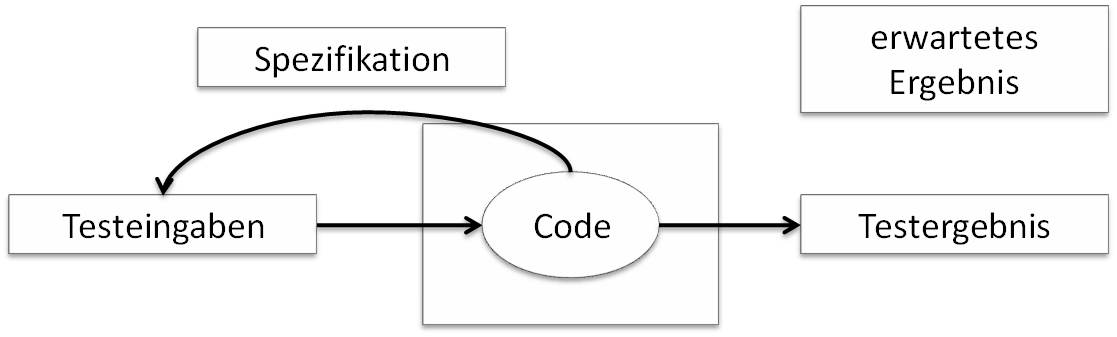
\includegraphics[scale=0.6]{img/codeBasedDesign.png}\\
  \footnotesize\sffamily\textbf{Quelle:} \cite[vgl. S. 19]{fewster_software_1999}
  \caption{Code-basierte Generierung von Testfällen}
  \label{fig:codeBasedDesign}
\end{figure}


\subsubsection{Interface-basierte Generierung von Eingabedaten}
\label{subsubsec:interfacebasierte_generierung}
Bei dieser Methode erfolgt die Generierung anhand von gut definierten Schnittstellen wie  der Benutzeroberfläche einer Desktop- oder Web-Anwendung (siehe Abbildung \ref{fig:interfaceBasedDesign}). 
Besteht die Oberfläche aus eine Reihe von Eingabeelementen kann zum Beispiel ein Testfall generiert werden, der jedes dieser Elemente überprüft. So kann beispielsweise getestet werden ob eine Checkbox nach dem Betätigen aktiviert bzw. deaktiviert wurde. Eine andere Möglichkeit wäre es rekursiv jeden Link in einer Webanwendung zu durchlaufen. Alle defekten Links einer Webanwendung können auf diese Weise identifiziert werden.
Mit Hilfe dieses Ansatzes ist es also auch möglich einfache Akzeptanzkriterien zu generieren. Werden die Links einer Web-Anwendung rekursiv durchlaufen, könnte beispielsweise überprüft werden, dass die Links auch auf eine neue Seite Führen. \cite[vgl. S. 20,21]{fewster_software_1999}

\begin{figure}[htb]
  \centering  
  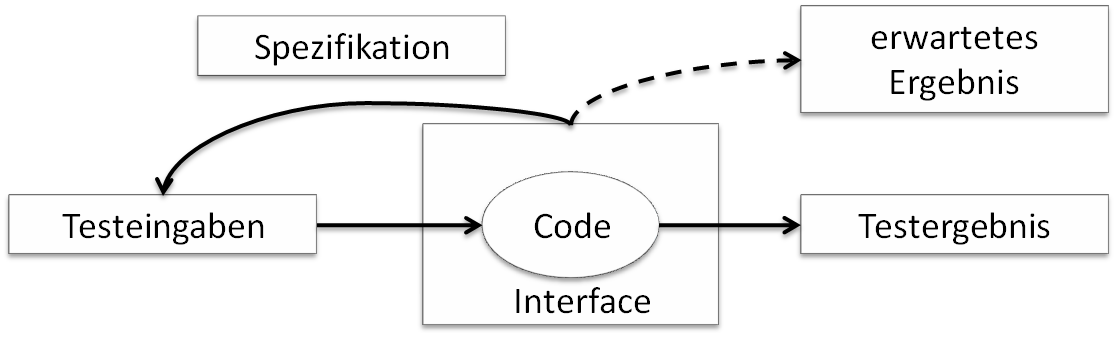
\includegraphics[scale=0.6]{img/interfaceBasedDesign.png}\\
  \footnotesize\sffamily\textbf{Quelle:} \cite[vgl. S. 20]{fewster_software_1999}
  \caption{Interface-basierte Generierung von Testfällen}
  \label{fig:interfaceBasedDesign}
\end{figure}


\subsubsection{Spezifikations-basierte Generierung von Eingabedaten}
\label{subsubsec:spezifikationsbasierte_generierung}
Mit Hilfe von Spezifikations-basierter Generierung ist es möglich sowohl Testeingaben als auch die zugehörigen erwarteten Ergebnisse zu erzeugen (siehe Abbildung \ref{fig:specBasedDesign}). Als Basis wird dazu eine Spezifikation benötigt die automatisiert analysiert werden kann. Die Möglichkeiten dafür reichen von natürlicher Sprache die gewissen Strukturen folgt bis hin zu technischen Modellen. Vor allem die Benutzung von Modellen hat in den letzten Jahren immer mehr an Bedeutung gewonnen und ist heute unter dem Namen modellbasiertes Testen bekannt. \cite{rossner_basiswissen_2010}
Ein Vorteil des Spezifikations-basierte Ansatzes ist es, dass die Testfälle nicht auf Basis einer Implementierung sondern auf Basis einer Spezifikation erzeugt werden. Damit ist sichergestellt, dass die Testfälle nicht nur, wie bei der Code-basierte Generierung, überprüfen \grq was die Software tut\grq , sondern \grq was sie tun soll\grq. \cite[vgl. S. 21]{fewster_software_1999}

\begin{figure}[htb]
  \centering  
  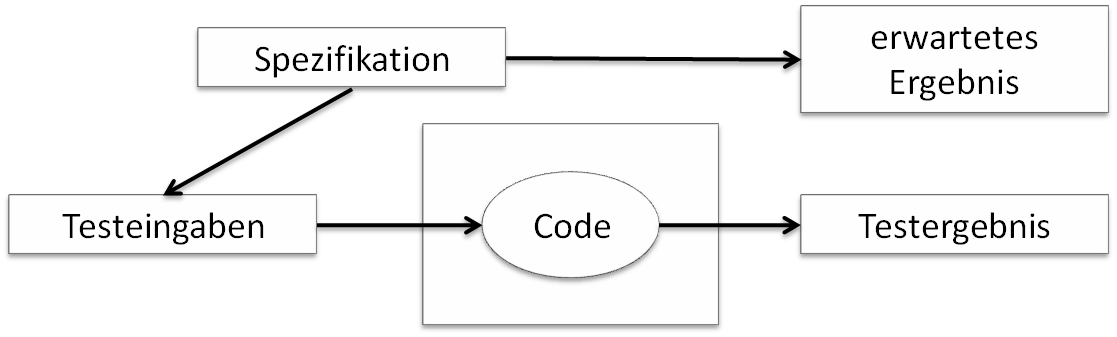
\includegraphics[scale=0.6]{img/specBasedDesign.png}\\
  \footnotesize\sffamily\textbf{Quelle:} \cite[vgl. S. 21]{fewster_software_1999}
  \caption{Spezifikations-basierte Generierung von Testfällen}
  \label{fig:specBasedDesign}
\end{figure}

\subsection{Testcodeerstellung}
\label{subsec:testcodeerstellung}
Bei der Testautomatisierung versteht man unter Testcodeerstellung das erzeugen von Testscripten bzw. Testcode, der später wiederholt gestartet werden kann. Der erzeugte Code setzt die Testfälle um die zuvor in der Designphase gefunden wurden.
In vielen Fällen handelt es sich dabei um einen manuellen Schritt. Die Testcodeerstellung ist oft eine reine Entwicklertätigkeit bei der ein Tester die angedachten Testfälle in Testcode implementiert.
Aber auch in diesem Schritt sind Möglichkeiten für eine Automatisierung gegeben.
Es existieren beispielsweise teilautomatisierte Ansätze. Mit Hilfe von sogenannten \grq record-and playback\grq\ Tools (R\&PB) können die Interaktionen eines Benutzers mit der zu testenden Software aufgezeichnet werden. Die aufgezeichneten Abläufe können dann verwendet werden um automatisierte Testskripte zu generieren.
Auch ein voll automatisierter Ansatz ist möglich wenn auch nicht so weit verbreitet wie der manuelle bzw. tailautomatisierte Ansatz.
Mittels modellbasiertem Testen ist es nicht nur möglich Testfalldesigns abzuleiten. Liegen die Modelle in einem entsprechend hohen Detailgrad vor ist es sogar möglich daraus direkt Testcode zu erzeugen. Bouquet et al. \cite{bouquet_test_2008} beschreiben beispielsweise einen modellbasierten Ansatz mit dessen Hilfe das designen, erstellen und ausführen von Testfällen automatisiert geschehen kann. \cite{amannejad_search-based_2014}
Zusammengefasst ist die Testcodeerstellung damit in drei unterschiedlichen Automatisierungsgraden möglich:
\begin{itemize}
\item Manuell
\item Teilautomatisiert (R\&PB)
\item Automatisiert
\end{itemize}

Allen Ansätzen gemeinsam ist, dass sie immer eine Schnittstelle zum System benötigen über welche der automatisierte Testcode mit der zu testenden Anwendung kommunizieren kann.
Meszaros et al. unterscheiden dazu zwei Hauptangriffspunkte:
\begin{itemize}
\item API: Als Schnittstelle wird der Code der zu testenden Anwendung direkt benutzt.
\item 
UI: Als Schnittstelle wird die Benutzeroberfläche der Anwendung verwendet.
\end{itemize}

Kombiniert man die verschiedenen Ansätze der Testcodeerstellung mit den Schnittstellen ergibt sich eine Matrix welche die verschiedenen Möglichkeiten der Testcodeerstellung beim automatisierten Testen abbildet. Eine grafische Darstellung dieser Matrix bietet Abbildung \ref{fig:bereicheTestcodeerstellung}.


\begin{figure}[htb]
  \centering  
  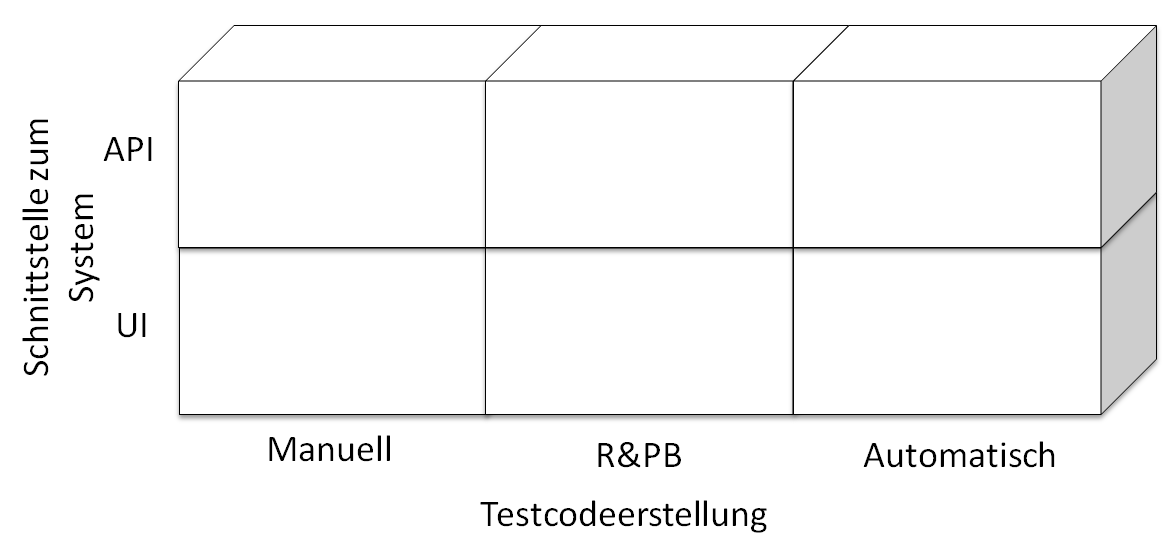
\includegraphics[scale=0.7]{img/bereicheTestcodeerstellung.png}\\
  \footnotesize\sffamily\textbf{Quelle:} vgl. \cite{fewster_software_1999}
  \caption{Verschiedene Möglichkeiten der Testcodeerstellung}
  \label{fig:bereicheTestcodeerstellung}
\end{figure}

Die vollautomatisierte Generierung befindet sich außerhalb des Rahmens dieser Arbeit und wird daher im folgenden nicht mehr näher betrachtet.
Meszaros et al. haben eine ähnliche Matrix aufgestellt die noch um eine weitere Dimension der Testgranularität (Unit-, Integrations- und System-Test) erweitert ist. Diese Dimension hat allerdings nur wenig Auswirkungen auf die Herangehensweise in der Testautomatisierung und wurden deshalb in Abbildung \ref{fig:bereicheTestcodeerstellung} nicht mit aufgeführt.

\subsubsection{API}
\label{subsubsec:API}

Unter der Abkürzung API (application programming interface) sind in diesem Zusammenhang alle Schnittstellen zu verstehen, die intern von der zu testenden Anwendung angeboten werden. Darunter fällt beispielsweise das direkte aufrufen von Servicemethoden die als Businesslogik innerhalb der Anwendung bereitgestellt werden.
Ein weit verbreitete Technologie die im Rahmen der Testautomatisierung oft diese Art der Schnittstelle verwenden sind die modernen \grq XUnit-Frameworks\grq. In den Meisten Programmiersprachen existiert ein Unit-Framework mit dem es möglich ist direkt die im Programm angebotene Logik mit automatisierten Testfällen abzuprüfen. In der Praxis wird diese Aufgabe meist direkt vom Entwickler in Form von Unit-Tests (Komponenten-Tests) übernommen. Der Begriff \grq XUnit-Frameworks\grq kann leicht missverstanden werden, da er impliziert, dass es sich bei den mit Hilfe des Frameworks umgesetzten Testfällen um Unit-Tests handelt. Tatsächlich können jedoch Testfälle aller Teststufen, von Unit- bis System-Test, mit Hilfe dieser Frameworks umgesetzt werden.
Die Testcodeerstellung erfolgt dabei meist Manuell womit diese Art der Automatisierung ein Beispiel für den oberen linken Quadranten in Abbildung \ref{fig:bereicheTestcodeerstellung} darstellt.







\subsection{Testdurchführung}
\label{subsec:testdurchführung}


\subsection{Testauswertung}
\label{subsec:testauswertung}



\section{Schnittstellen der Testautomatisierung zum System}
\label{sec:schnittstellen_der_testautomatisierung_zum_syste}

Jeder testfall muss in irgendeiner weise mit dem zu testenden objekt interagieren.
Analog zu manuellen tests gibt es hierfür verschiedene möglichkeiten.
\subsection{API}
\subsubsection{JUnit}
\label{sec:junit}

\subsection{GUI}
Web
